\documentclass[preprint]{aastex}
%\documentclass{emulateapj}


% has to be before amssymb it seems
%\usepackage{color,hyperref}
%\definecolor{linkcolor}{rgb}{0,0,0.5}
%\hypersetup{colorlinks=true,linkcolor=linkcolor,citecolor=linkcolor,
%            filecolor=linkcolor,urlcolor=linkcolor}
%\usepackage{amssymb,amsmath}

\usepackage{color}
\usepackage{url}
\usepackage{graphicx}
\graphicspath{{figures/}}

% For Python code
\usepackage{listings}
\definecolor{lbcolor}{rgb}{0.9,0.9,0.9}
\lstset{language=Python,
        basicstyle=\footnotesize\ttfamily,
        showspaces=false,
        showstringspaces=false,
        tabsize=2,
        breaklines=false,
        breakatwhitespace=true,
        identifierstyle=\ttfamily,
        keywordstyle=\bfseries\color[rgb]{0.133,0.545,0.133},
        commentstyle=\color[rgb]{0.133,0.545,0.133},
        stringstyle=\color[rgb]{0.627,0.126,0.941},
    }

% Draft watermark:
%\usepackage{draftwatermark}
%\SetWatermarkLightness{0.9}
%\SetWatermarkScale{4}

\usepackage{amsmath}
\DeclareMathOperator{\sinc}{sinc}
\DeclareMathOperator{\III}{III}

% Some macros
\newcommand{\todo}[1]{{\color{red} [TODO: #1]}}
\newcommand{\foreign}[1]{{\it #1}}

\newcommand{\apriori}{\foreign{a priori}}
\newcommand{\adhoc}{\foreign{ad hoc}}
\newcommand{\etal}{\foreign{et\,al.}}
\newcommand{\etc}{\foreign{etc.}}

\newcommand{\Fig}[1]{Figure~\ref{fig:#1}}
\newcommand{\fig}[1]{\Fig{#1}}
\newcommand{\figlabel}[1]{\label{fig:#1}}
\newcommand{\Eq}[1]{Equation~(\ref{eq:#1})}
\newcommand{\eq}[1]{\Eq{#1}}
\newcommand{\eqs}[2]{Equations~(\ref{eq:#1})-(\ref{eq:#2})}
\newcommand{\eqlabel}[1]{\label{eq:#1}}
\newcommand{\Sect}[1]{Section~\ref{sect:#1}}
\newcommand{\sect}[1]{\Sect{#1}}
\newcommand{\sects}[1]{Sections~#1}
\newcommand{\App}[1]{Appendix~\ref{sect:#1}}
\newcommand{\app}[1]{\App{#1}}
\newcommand{\sectlabel}[1]{\label{sect:#1}}

\usepackage[normalem]{ulem}
\newcommand{\new}[1]{{\color{red} #1}}
\newcommand{\old}[1]{{\sout{#1}}}


\begin{document}

\title{Understanding the Lomb-Scargle Periodogram}

\newcommand{\escience}{*}
\newcommand{\uwastro}{+}
\author{Jacob T. VanderPlas\altaffilmark{\escience}}
\altaffiltext{\escience}{eScience Institute, University of Washington}


\begin{abstract}
This paper gives an introduction to the practical aspects of the use of Lomb-Scargle periodograms and related algorithms to detect periodic signals.
Rather than a rigorous mathematical treatment, the goal of this paper is to build intuition about what assumptions are baked into any periodogram computation.
We discuss... and ... and ...
\end{abstract}

\keywords{
    methods: data analysis ---
    methods: statistical
}

\section{Introduction}
\sectlabel{introduction}

\begin{figure}[ht]
\centering
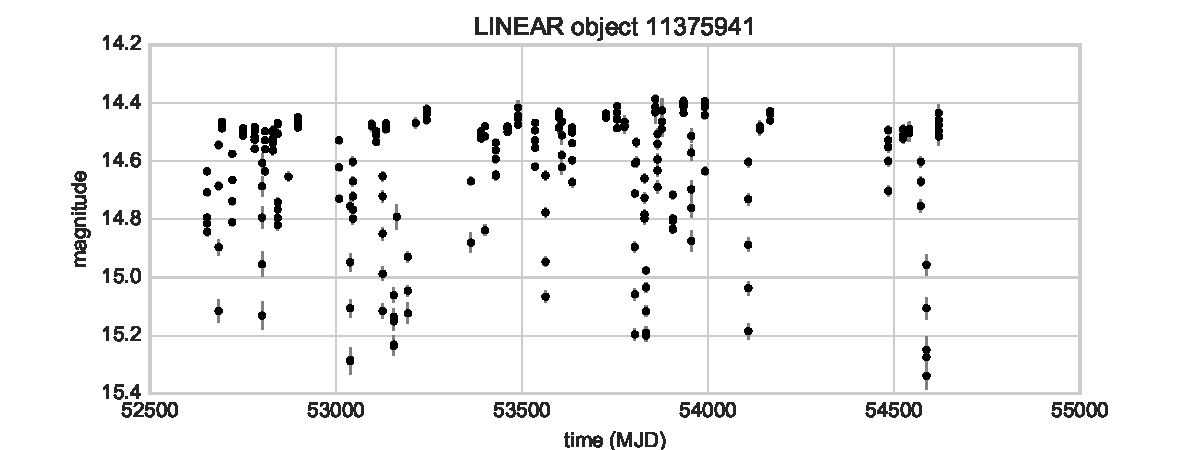
\includegraphics[width=\textwidth]{fig01_LINEAR_data}
\caption{Observed light curve from LINEAR object ID 11375941. Uncertainties
  are indicated by the gray errorbars on each point.
  \figlabel{LINEAR_data}
}
\end{figure}


\begin{figure}[ht]
\centering
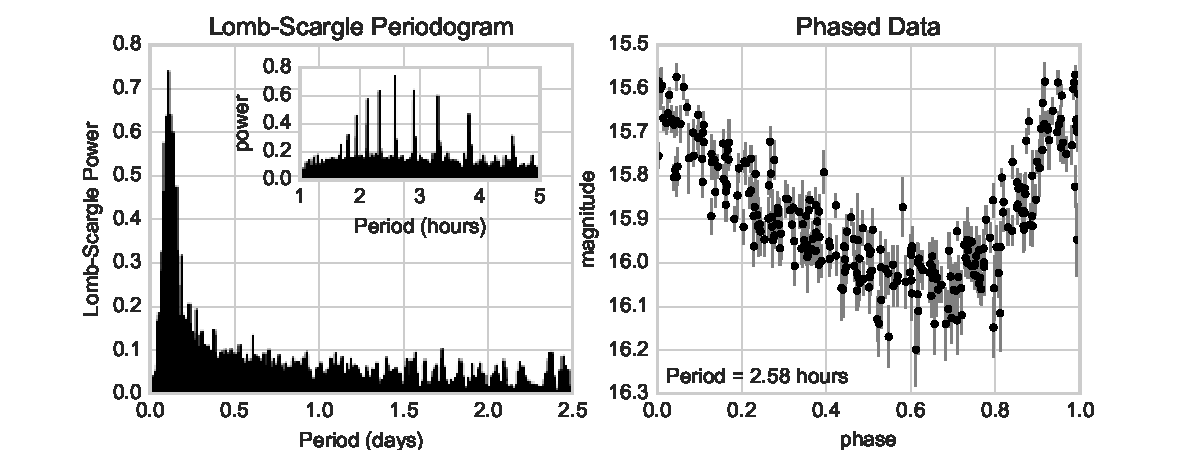
\includegraphics[width=\textwidth]{fig02_LINEAR_PSD}
\caption{{\it Left panel:} the Lomb-Scargle periodogram computed from the data
    shown in \fig{LINEAR_data}, with an inset detailing the region near the peak.
    {\it Right panel:} the input data in \fig{LINEAR_data}, folded over the
    detected 2.58-hour period to show the coherent periodic variability.
    \figlabel{LINEAR_power}
}
\end{figure}

The Lomb-Scargle periodogram \citep{Lomb76, Scargle82}
is a well-known algorithm for detecting periodicity
in unevenly-sampled time-series, particularly within the astronomy community.
For example, consider the data shown in \fig{LINEAR_data}.
This is an irregularly-sampled timeseries showing a single object from the
LINEAR survey \citep{LINEAR1, LINEAR3}, with magnitude measured 280 times over the
course of five and a half years\footnote{
  Python code to reproduce \fig{LINEAR_data}, as well as all other figures
  in this manuscript, is available at 
  \url{http://github.com/jakevdp/PracticalLombScargle/}}.

By eye, it is clear that the brightness of the object varies in time with a range spanning approximately 0.8 magnitudes, but what is not immediately clear is that this variation is periodic in time.
The Lomb-Scargle periodogram is a method that allows efficient computation of a Fourier-like power spectrum from such unevenly-sampled data, resulting in an intuitive means of determining the period of oscillation.

The left panel of \fig{LINEAR_power} shows the Lomb-Scargle periodogram computed for the data in \fig{LINEAR_data}.
Computing the Lomb-Scargle periodogram for the data gives us a measure of the
power as a function of period of oscillation (\fig{LINEAR_power}, left), from
which we can determine the period of oscillation of approximately 2.58 hours.
The right panel of \fig{LINEAR_power} shows a folded visualization of
the same data as \fig{LINEAR_data} -- i.e.{} plotted as a function of phase
rather than time.\footnote{
    The periodogram in \fig{LINEAR_power} was computed using
    {\tt astropy.stats.LombScargle}
    from the AstroPy project; see \url{http://astropy.org/}.
}

Often this is exactly how the Lomb-Scargle periodogram is presented: as a clean, well-defined procedure to detect the periodic component in an unevenly-sampled dataset.
In practice, however, there are a number of subtle issues that must be considered when applying a Lomb-Scargle analysis to real-world datasets, and I have found that these are rarely presented together at an introductory level.
Here are a few questions in particular that we might wish to ask about the results in \fig{LINEAR_power}:
\begin{enumerate}
  \item What is the source of the multiple peaks revealed by the Lomb-Scargle Periodogram?
  \item What is a suitable range of frequencies to search for a given dataset?
  \item What is the Nyquist frequency for this type of analysis?
  \item How should we choose the spacing of the frequency grid for our periodogram?
  \item How should we understand the uncertainty of the computed frequency?
  \item What assumptions is the Lomb-Scargle periodogram making about the signal?
\end{enumerate}
Questions like these are discussed in various textbooks and review papers, but I have not come across any concise reference that discusses such questions in depth.
This paper seeks to fill that gap, and provide a practical, semi-technical guide to the effective use of the Lomb-Scargle method of periodic analysis.
This paper does not seek a complete or rigorous treatment of the mathematics involved, but rather seeks to develop the intuition of {\it how} to think about the issues involved.


\section{Background: the Continuous Fourier Transform}

In order to understand how we should interpret the Lomb-Scargle periodogram, we will first briefly step back and review the subject of Fourier analysis of continuous signals.
Consider a continuously-defined signal $g(t)$.
Its Fourier transform is given by the following integral:
\begin{equation}
    \hat{g}(f) \equiv \int_{-\infty}^\infty g(t) e^{-2\pi i f t} dt
    \eqlabel{FT-def}
\end{equation}
The inverse relationship is given by:
\begin{equation}
    g(t) \equiv \int_{-\infty}^\infty \hat{g}(f) e^{+2\pi i f t} df
    \eqlabel{IFT-def}
\end{equation}
For convenience we will also define the Fourier transform operator
$\mathcal{F}$, such that
\begin{eqnarray}
    \mathcal{F}\{g\} &=& \hat{g} \\
    \mathcal{F}^{-1}\{\hat{g}\} &=& g
\end{eqnarray}
As a further shorthand, we'll sometimes use a double arrow to denote a Fourier
pair; for example
\begin{equation}
  g(x) \Longleftrightarrow \hat{g}(f).
\end{equation}

\subsection{Properties of the Fourier Transform}

The continuous Fourier transform has a number of useful properties that we will make use of in our discussion.

\begin{description}
   \item[The Fourier transform is a linear operation.]
     That is, for any constant $A$ and any functions $f$ and $g$, we can write
     \begin{eqnarray}
       \mathcal{F}\{f(t) + g(t)\} &=& \mathcal{F}\{f(t)\} + \mathcal{F}\{g(t)\}\nonumber\\
       \mathcal{F}\{A f(t)\} &=& A\mathcal{F}\{f(t)\}
     \end{eqnarray}
     which follows from the linearity of the Fourier integral.

   \item[The Fourier transform of sinusoid with frequency $f_0$ is a sum of delta functions at $\pm f_0$.]
     Given the integral definition of the Dirac delta function, it is straightforward to show that
     \begin{equation}
       \mathcal{F}\{e^{2\pi f_0 t}\} = \delta(f - f_0).
       \eqlabel{delta_FT}
     \end{equation}
     Euler's formula shows how such a complex exponential
     can be expressed in terms of sines and cosines:
     \begin{equation}
       e^{2\pi f_0 t} = \cos(2\pi f_0 t) + i\sin(2\pi f_0 t).
       \eqlabel{Euler_formula}
     \end{equation}
     Using the linearity of the Fourier transform, we can take these identites
     and derive the following identities:
     \begin{eqnarray}
       \mathcal{F}\{\cos(2\pi f_0 t)\} &=& \frac{1}{2}\left[\delta(f - f_0) + \delta(f + f_0)\right]\nonumber\\
       \mathcal{F}\{\sin(2\pi f_0 t)\} &=& \frac{1}{2i}\left[\delta(f - f_0) - \delta(f + f_0)\right].
     \end{eqnarray}
     In other words, a sinusoidal signal with frequency $f_0$ has a Fourier transform consisting of a weighted sum of delta functions at $\pm f_0$.

   \item[A time-shift imparts a phase in the Fourier transform.]
     Given a well-behaved function $g(t)$ we can use a transformation of
     variables to derive the following identity:
     \begin{equation}
       \mathcal{F}\{g(t - t_0)\} = \mathcal{F}\{g(t)\} e^{-2\pi i ft_0}
     \end{equation}
     The key observation here is that the time-shift does not change the
     amplitude of the resulting transform, but only the phase.
\end{description}
These properties taken together make the Fourier transform quite useful for the study of periodic signals.
The linearity of the transform means that any signal made up of a sum of periodic components will have a Fourier transform consisting of a sum of delta functions at those frequencies: that is, the Fourier transform is a {\it direct} measure of the periodic content of a function.

Further, if we compute the squared amplitude of the resulting transform, we can both do away with complex components and remove the phase imparted by any time offsets; this squared amplitude is usually known as the {\it Power Spectrum}:
\begin{equation}
  \mathcal{P}\{g\} \equiv \left|\mathcal{F}\{g\}\right|^2
  \eqlabel{power-spectrum}
\end{equation}
The power spectrum of a function is a positive real-valued function of $f$ that quantifies the contribution of each frequency $f$ to the total signal.

\subsection{Some Useful Fourier Pairs}

\begin{figure}[ht]
\centering
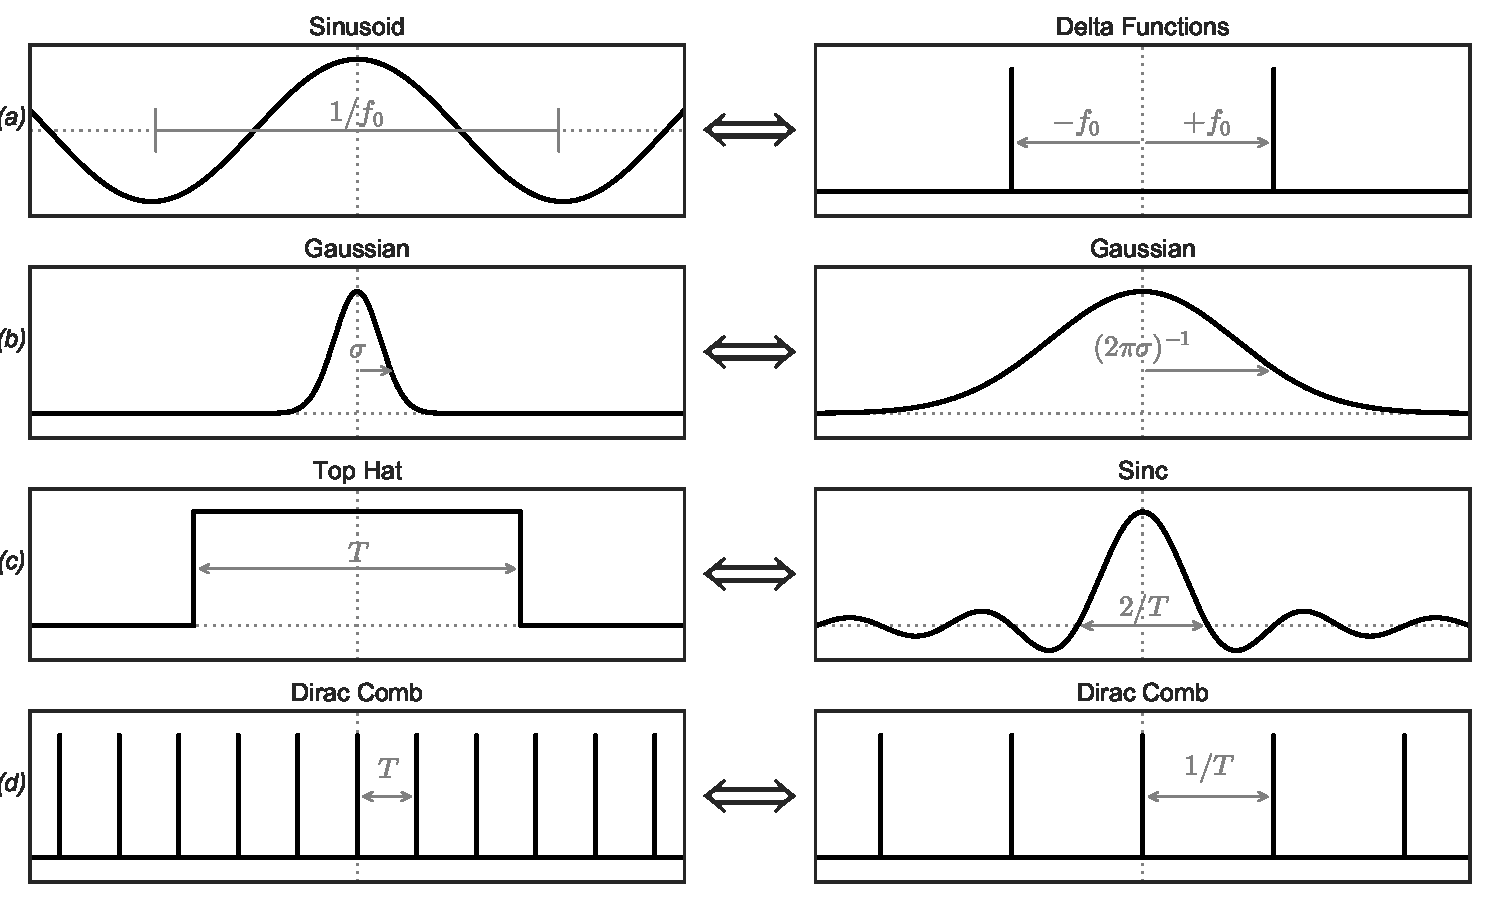
\includegraphics[width=\textwidth]{fig03_Fourier_pairs}
\caption{Visualization of important Fourier pairs.\figlabel{fourier_pairs}}
\end{figure}

We have already discussed that the Fourier transform of a complex exponential is a single delta function.
This is just one of many ``Fourier Pairs'' to keep in mind as we progress to understanding the Lomb-Scargle Periodogram.
We list a few more important pairs here (see \Fig{fourier_pairs} for a visual representation of the following pairs):


\begin{description}
  \item[The Fourier transform of a sinusoid is a pair of Delta functions.]
    (See \fig{fourier_pairs}{\it a})
    \begin{equation}
      \mathcal{F}\{\cos(2\pi f_0 t)\} = \frac{1}{2}\left[\delta(f-f_0) + \delta(f+f_0)\right]
    \end{equation}
    We saw this above, but repeat it here for completeness.

   \item[The Fourier transform of a Gaussian is a Gaussian.]
    (See \fig{fourier_pairs}{\it b})
     \begin{equation}
       \mathcal{F}\{{\rm N}(t; \sigma)\} = \frac{1}{\sqrt{2\pi\sigma^2}}{\rm N}\left(f;\frac{1}{2\pi\sigma}\right)
     \end{equation}
     The Gaussian function ${\rm N}(t, \sigma)$ is given by
     \begin{equation}
       {\rm N}(t; \sigma) \equiv \frac{1}{\sqrt{2\pi\sigma^2}}e^{-t^2/(2\sigma^2)}
     \end{equation}

  \item[The Fourier transform of a tophat function is a sinc function.]
    (See \fig{fourier_pairs}{\it c})
    \begin{equation}
      \mathcal{F}\{\Pi_T(t)\} = \sinc(f T)
    \end{equation}
    The tophat function, $\Pi_T(t)$, is a normalized symmetric function that
    is uniform within a range given by $T$, and zero elsewhere:
    \begin{equation}
      \Pi_T(t)  \equiv \left\{
      \begin{array}{ll}
        1 / T, & |t| \le T / 2 \\
        0,     & |t| > T / 2
      \end{array}
      \right.
    \end{equation}
    The sinc function is given by the standard definition:
    \begin{equation}
      \sinc(x) \equiv \frac{\sin(\pi x)}{\pi x}
    \end{equation}

  \item[The Fourier transform of a Dirac comb is a Dirac comb.]
    (See \fig{fourier_pairs}{\it d})
    \begin{equation}
      \mathcal{F}\{\III_T(t)\} = \frac{1}{T}\III_{1/T}(f)
    \end{equation}
    The Dirac comb, $\III_T(t)$, is an infinite sequence of Dirac delta functions placed at even intervals of size $T$:
    \begin{equation}
      \III_T(t) \equiv \sum_{n=-\infty}^\infty \delta(t - nT)
      \eqlabel{dirac_comb}
    \end{equation}
\end{description}
The key observation in each of these Fourier pairs is the reciprocity
of scales between a function and its Fourier transform:
that is, a function with a characteristic scale $T$ will in general
have a Fourier transform with characteristic scale of $1/T$.
This feature will turn out to be very important as we push further in
understanding the Lomb-Scargle Periodogram.


\subsection{The Convolution Theorem}

A final property of the Fourier transform that we will discuss here is its
ability to convert convolutions into point-wise products.
A convolution of two functions, usually denoted with a $\ast$, is defined
as follows:
\begin{equation}
  [f \ast g](t) = \int_{-\infty}^\infty f(\tau)g(t - \tau) d\tau
  \eqlabel{convolution_definition}
\end{equation}
From the definition, it is clear that a convolution amounts to ``sliding'' one
function past the other.
Such an operation is commonly used, for example, in smoothing a function,
as visualized in \Fig{convolution} for a tophat-shaped smoothing window.

\begin{figure}[ht]
  \centering
  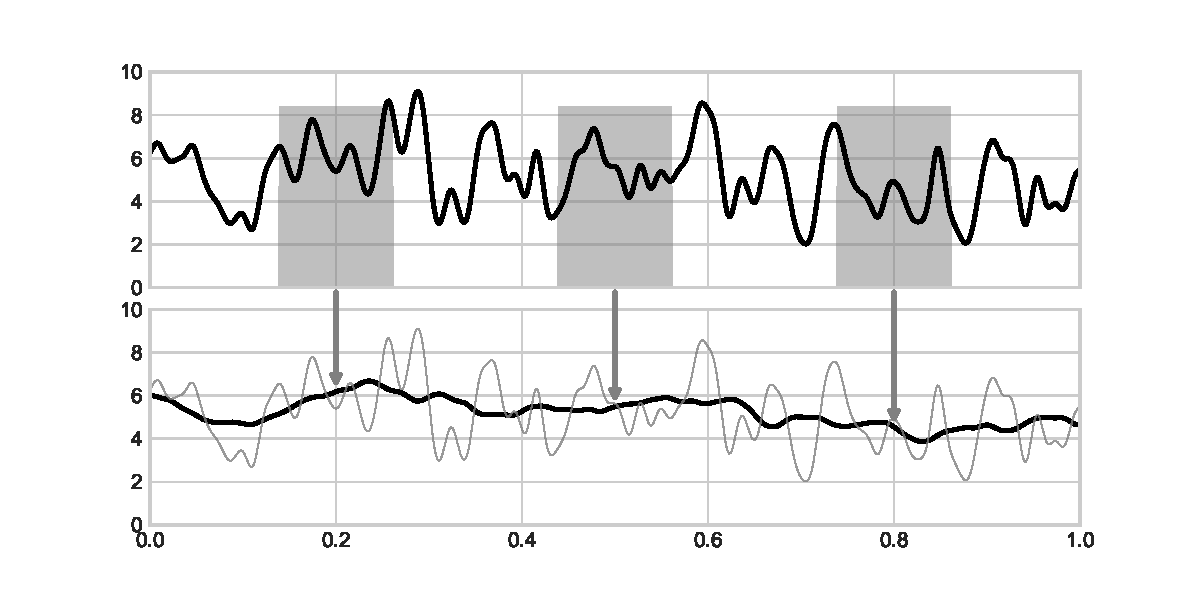
\includegraphics[width=\textwidth]{fig04_Convolution_Diagram}
  \caption{Visualization of a convolution between a continuous signal and a tophat smoothing kernel.
    The normalized tophat-shaped window function slides across the domain (upper panel),
    such that at each point the mean of the values within the window are
    used to compute the smoothed function (lower panel).
    \figlabel{convolution}}
\end{figure}

Given this definition of a convolution, it can be shown that the Fourier transform of a convolution is the point-wise product of the Fourier transforms:
\begin{equation}
  \mathcal{F}\{f \ast g\} = \mathcal{F}\{f\} \cdot \mathcal{F}\{g\}
  \eqlabel{convolution_theorem}
\end{equation}
In practice, this is a much more efficient means of computing the convolution
than to directly solve at each time $t$ the integral over $\tau$ that appears
in \eq{convolution_definition}.
This result in \eq{convolution_theorem} is known as the
{\it convolution theorem}, and is illustrated in \fig{convolution_theorem}.
\begin{figure}[ht]
  \centering
  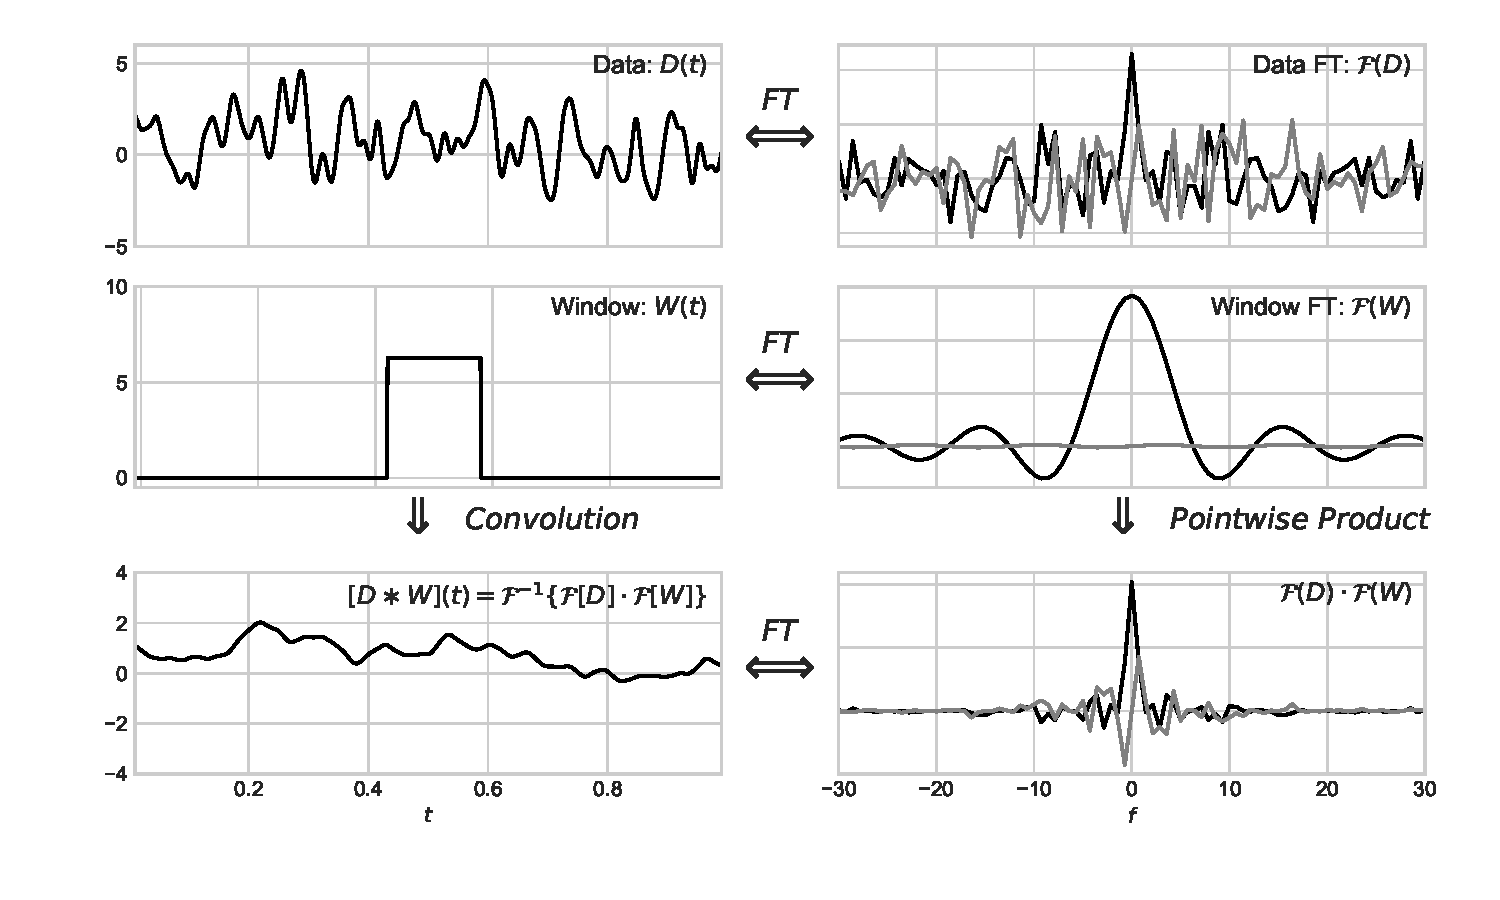
\includegraphics[width=\textwidth]{fig05_Convolution_Theorem}
  \caption{Visualization of the convolution theorem (\eq{convolution_theorem}).
    The key is that the Fourier transform of
    a convolution is the pointwise product of the two Fourier transforms.
    In the right panels, the black and gray lines represent the real and
    imaginary part of the transform, respectively.
    \figlabel{convolution_theorem}}
\end{figure}
When thinking about frequency components of time-domain measurements, this
property of the Fourier transform becomes essential, as we will see.

An important corrollary is that the Fourier transform of a product is a convolution of the two transforms:
\begin{equation}
  \mathcal{F}\{f \cdot g\} = \mathcal{F}\{f\} \ast \mathcal{F}\{g\}
  \eqlabel{convolution_theorem_inverse}
\end{equation}
We will explore the impact of this in the next section.

\section{Window Functions: From Idealized to Real-world signals}
In a typical observational setting, we will be observing some small part of
a larger time-varying signal.
For example, if you have a very long signal that you measure for a finite
amount of time, your measurement is a point-wise product between the true
signal and a suitable tophat function describing your measurement process.
If you have a continuous signal that you measure at regular intervals, your
measurement is a point-wise product between the true signal and an appropriate
Dirac comb describing your measurement process.
From what we learned about the convolution theorem in the previous section, it
is clear that {\it the measured Fourier transform will be the true transform
convolved with the transform of the obverving window}.
This has some interesting consequences, as we shall see.

\subsection{Effect of a Tophat Window}
First, let's consider the case of observing a continuous periodic signal over
a limited span of time, as illustrated in \Fig{tophat_window}.
Here we consider a periodic function made up of three frequency components, observed within a 10-unit time window.
The observed signal in this case can be thought of as a pointwise product of an infinite periodic signal, and a tophat window function.
Using \eq{convolution_theorem_inverse}, we see that the Fourier transform of
this function is equivalent to the convolution of the Fourier transforms of each component, which are a set of delta functions and a sinc function, respectively.
For a purely periodic signal, this convolution has the effect of broadening the delta functions representing the signal, turning each of them into a shifted sinc function.
Because of the inverse relationship between the width of the window and the width of its transform (see \Fig{fourier_pairs}), it follows that a wider observing window leads to proportionally less spread in the Fourier transform of the observed function.

\begin{figure}[ht]
  \centering
  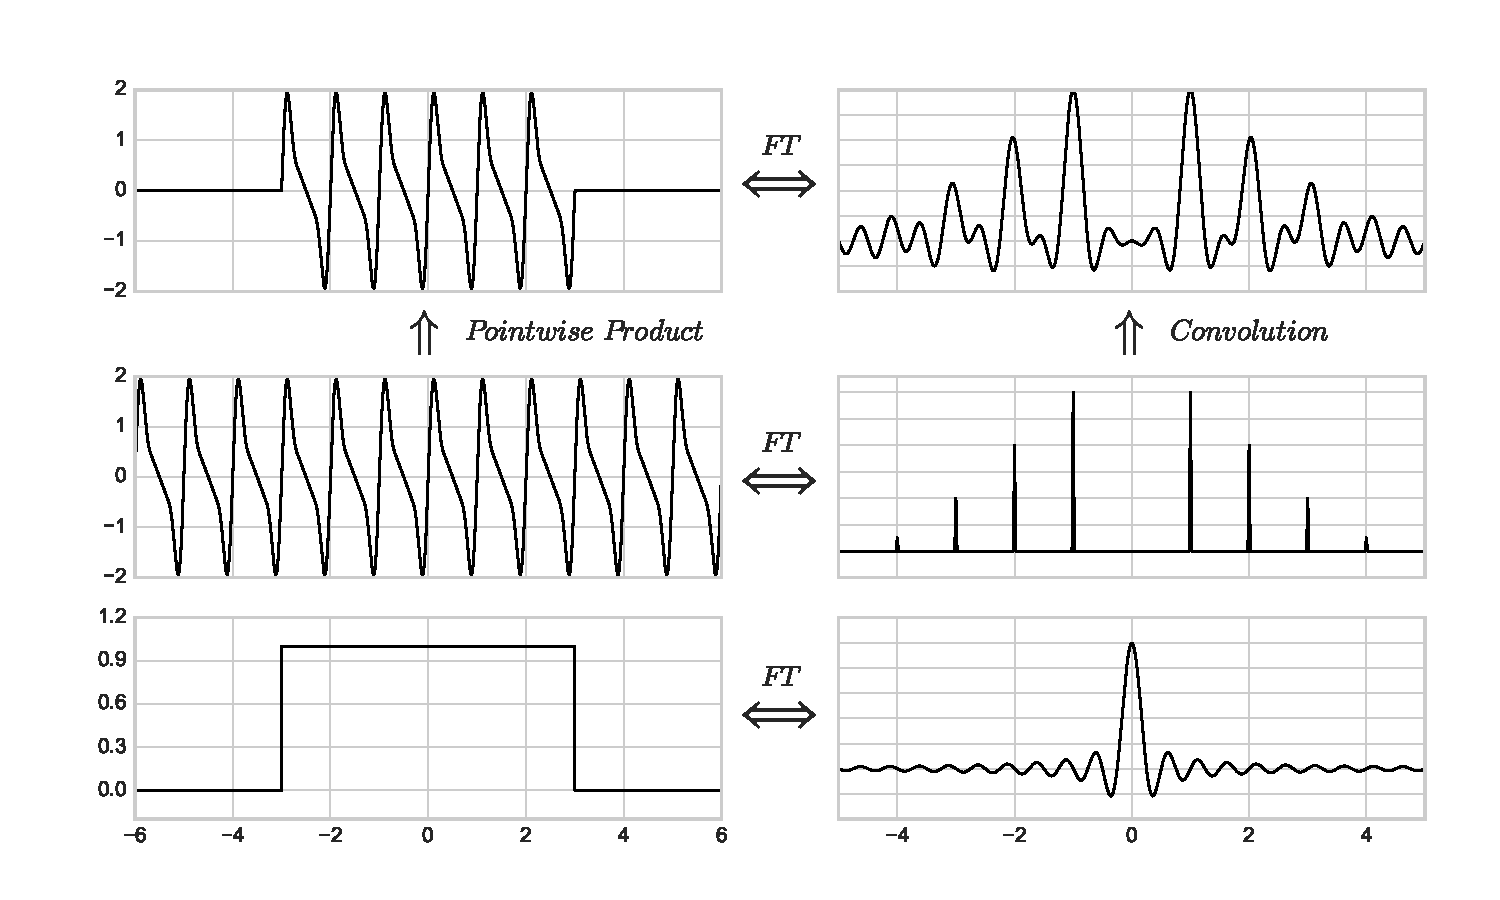
\includegraphics[width=\textwidth]{fig06_Tophat_Window}
  \caption{Visualization of the effect on the Fourier transform of a
    tophat-shaped observing window (i.e., a continuous signal observed
    fully, but only within a finite range of time). The observed Fourier
    transform is a convolution of the true transform (here a series of Delta
    functions) and the window transform (here a narrow sinc function).
    \figlabel{tophat_window}}
\end{figure}

\subsection{The Dirac Comb and the Discrete Fourier Transform}
Another window function that commonly arises is when a continuous signal is
sampled instantaneously at regular intervals.
Such an observation is, in effect, a point-wise product between the true
underlying signal and a Dirac comb with the $T$ parameter matching the spacing
of the observations; this is illustrated in \fig{comb_window_1}.

\begin{figure}[ht]
  \centering
  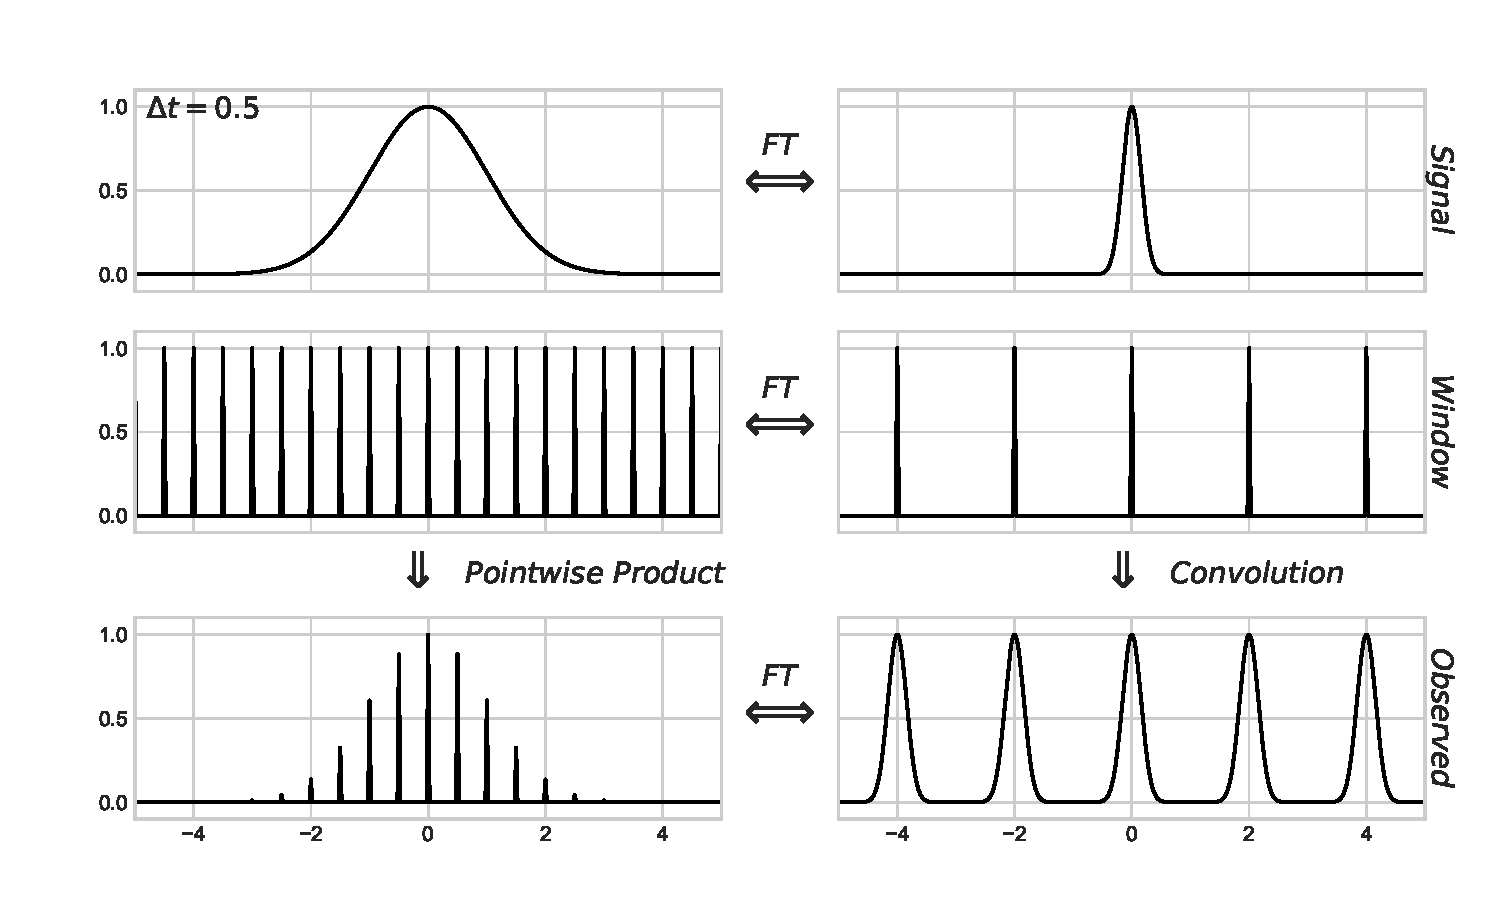
\includegraphics[width=\textwidth]{fig07_comb_window_1}
  \caption{Visualization of the effect on the Fourier transform of a
    Dirac Comb observing window (i.e., a long string of evenly-spaced
    discrete observations). The observed Fourier
    transform is a convolution of the true transform (here a localized
    Gaussian) and the window transform (here another Dirac comb).
    \figlabel{comb_window_1}}
\end{figure}

Interestingly, because the Fourier transform of a Dirac comb is another Dirac
comb, the effect of such an observing window is to create a long sequence
of aliases with a spacing of $1/T$.
With this in mind, we can be assured in this case that evaluating the
transform in the range $(2T)^{-1} \le f < (2T)^{-1}$ is sufficient to capture
all the available frequency information:
the signal outside that range is a sequence of identical aliases of
what lies in that range.
In fact, due to the nature of the aliasing, it is in fact sufficient to
compute the transform in {\it any} range of width $1/T$, and it is often
convenient to instead use the range $0 \le f < 1/T$.

\subsubsection{The Nyquist Limit}

The example in \fig{comb_window_1} is somewhat of a best-case scenario, because
the true Fourier transform values lie entirely in a range of width $1/T$.
If we change the sampling rate so that this is no longer the case, we will
have a situation similar to that in \fig{comb_window_2}.
With a lower sampling rate, the signal transform no longer fits within the
frequency window, and the true Fourier transform {\it cannot be recovered}
from the observed transform.

This implies that if we have a regularly-sampled function with a sampling
rate of of $f_0 = 1/T$, we can only fully recover the freuqency information
if the signal is {\it band-limited} between frequencies $\pm f_0/2$.
This is one way to motivate the famous Nyquist sampling limit, which says
that to fully represent the frequency content of a ``band-limited signal''
with all Fourier power in the range $\pm B$, we must sample the data with a
rate of at least $2B$.

\begin{figure}[ht]
  \centering
  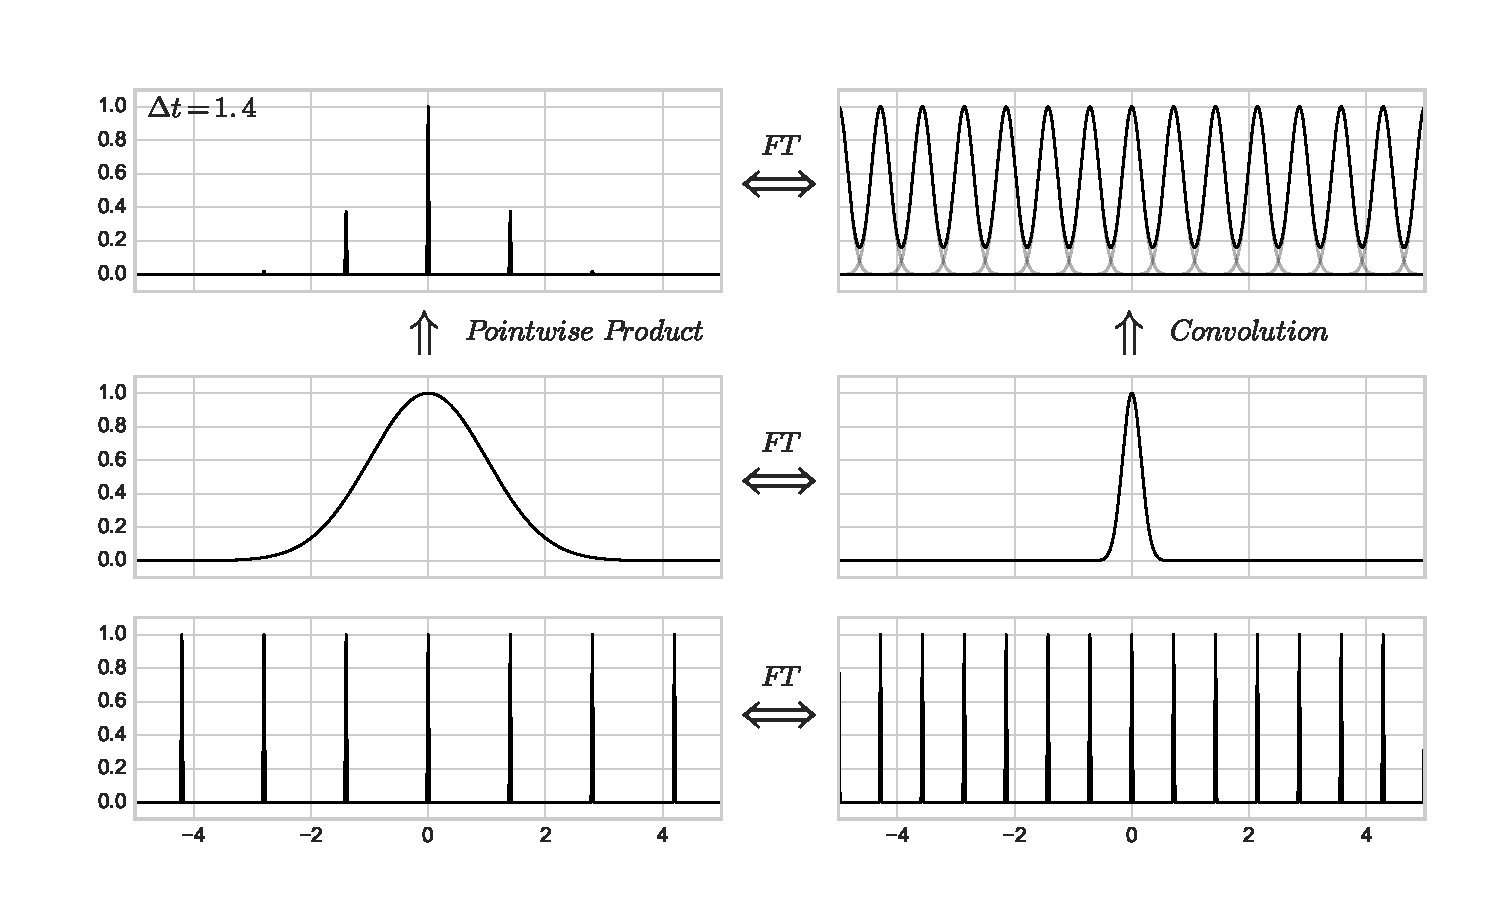
\includegraphics[width=\textwidth]{fig08_comb_window_2}
  \caption{Repeating the visualization from \fig{comb_window_1}, but here with
    a lower sampling rate. The result is that the Fourier transform of the
    window function (lower left) has spacing narrower than the Fourier transform
    of the signal (middle left), meaning the observed Fourier transform has
    aliasing of signals, such that not all frequency information can be
    recovered.
    \figlabel{comb_window_2}}
\end{figure}

\subsubsection{The Discrete Fourier Transform}
For regularly-spaced observations defined by a Dirac comb, the delta functions
serve to collapse the Fourier integral into a sum over periodic components.
Suppose we have a true (infinitely long and continuous) signal $g(t)$, but
we observe it only at a regular grid with spacing $T$. In this case, our
observed signal is $g_{obs} = g(t) \III_T(t)$ and its Fourier transform is
\begin{equation}
  \hat{g}_{obs}(f) = \sum_{n=-\infty}^\infty g(nT) e^{-2\pi i f n T},
\end{equation}
which follows directly from \eq{FT-def} and \eq{dirac_comb}.

In the real world, however, we will not have an infinite number of observations,
but rather a finite number of samples $N$.
We can choose the coordinate system appropriately and define
$g_n \equiv g(nT)$ to write
\begin{equation}
  \hat{g}_{obs}(f) = \sum_{n=0}^N g_n e^{-2\pi i f n T}
  \eqlabel{DFT_f}
\end{equation}
From the arguments around Nyquist aliasing, we know that the only relevant
frequency range is from $0 \le f \le 1/T$, and so we can define $N$
evenly-spaced frequencies with $\Delta f = 1 / (NT)$ covering this range.
Denoting the sampled transform as
$\hat{g}_k \equiv \hat{g}_{obs}(k\Delta f)$, we can write
\begin{equation}
  \hat{g}_k = \sum_{n=0}^N g_n e^{-2\pi i k n / N}
  \eqlabel{DFT}
\end{equation}
which you might recognize as the standard form of the discrete Fourier
transform.

You may have noticed we glossed over something here: the effect of switching
from an infinite number of samples to a finite number of samples.
In moving from $\hat{g}^{(T)}$ to $\hat{g}^{(N,T)}$, we have effectively applied
to our data a rectangular window function of width $NT$.
From the discussion accompanying \fig{tophat_window}, we know what this does:
it gives us a Fourier transform convolved with a sinc function of width
$1 / (NT)$, resulting in the ``smearing'' of the Fourier transform signal
with this width.
Roughly speaking, then, any two Fourier transform values at frequencies within
$1/(NT)$ of each other will not be independent, and so we should space our
evaluations of the frequency with $\Delta f \ge 1/(NT)$.
Comparing to above, we see that this is {\it exactly the frequency spacing}
we arrived at from Nyquist-frequency arguments.

What this indicates is that the frequency spacing of the discrete Fourier
transform is optimal in terms of both the Nyquist sampling limit
{\it and} the effect of the finite observing window!
Now, this argument has admittedly been a bit hand-wavy, but there do exist
mathematically rigorous approaches to proving that the discrete Fourier
transform in \eq{DFT} captures all of the available frequency information
for a uniformly-sampled function $g_n$
\citep[see, e.g.][]{FoundationsOfSignalProcessing}.
Despite the semi-qualitative nature of our discussion,
I find it to be a helpful approach
in developing intuition regarding the relationship between the
continuous and discrete Fourier transforms.

\subsubsection{The Schuster Periodogram}

With the discrete Fourier transform defined in \eqs{DFT_f}{DFT}, we can
apply the definition of the Fourier power spectrum from \eq{power-spectrum}
to compute the {\it Schuster Periodogram}, first proposed by \citet{Schuster98}:
\begin{equation}
  P_S(f) = \frac{1}{N}\left|\sum_{n=1}^N g_n e^{-2\pi i f t_n}\right|^2
  \eqlabel{schuster-periodogram}
\end{equation}
Apart from the $1/N$ scaling, this is precisely the Fourier power defined
in \eq{power-spectrum} for the expression in \eq{DFT_f}, and it follows that
for a uniformly-sampled function $g_n$, the Schuster periodogram captures
all of the relevant frequency information present in the data.

\todo{Add simulated RR Lyrae data and show the Shuster periodogram}


\section{Non-uniform Sampling Windows}

In the real world, particularly in fields like Astronomy where observations are
subject to interruptions from weather and diurnal cycles, the sampling rate
is generally far from uniform.
Using the same approach as we used to explore uniform sampling in the previous
section, we can now explore non-uniform sampling here.

In the general non-uniform case, we measure some signal at a set of $N$ times
which we will denote $\{t_n\}$.
Our observing window function in this case is still a sum of delta functions,
but at non-uniform locations.
Mathematically, the observing window will look like this:

\begin{equation}
W(t; \{t_n\}) = \sum_{n=1}^{N} \delta(t - t_n)
\end{equation}

Applying this window to our true underlying signal $g(t)$, we find an observed
signal of the form:

\begin{eqnarray}
  g_{obs}(t) &=& g(t) W(t; \{t_n\}) \nonumber\\
             &=& \sum_{n=1}^{N} g(t_n)\delta(t - t_n)
  \eqlabel{g-nonuniform}
\end{eqnarray}

Just as in the uniform case, the observed signal is a convolution of the true
signal transform and the window transform; unlike in the uniform case, the
window transform will generally {\it not} be a nice clean function.
\Fig{random_window} shows the effect on the Fourier transform of a
non-uniform observing cadence with a sampling rate identical to that
in \fig{comb_window_1}.

A few things stand-out in this figure. In particular, the Fourier transform of
the non-uniformly spaced delta functions looks like random noise, and in some
senses it is: the Fourier space representation reflects the frequency of
observations, and so non-structured spacing of observations will lead to
a non-structured Fourier representation of the window function.
This non-structured window transform, when convolved with the Fourier transform
of the true signal, results in an observed Fourier transform with the same
lack of useful structure.
Unlike the uniform result in \Fig{comb_window_1}, there is no direct aliasing
of the true signal, and no way to exactly recover any portion of the true
Fourier transform of this data.


\begin{figure}[ht]
  \centering
  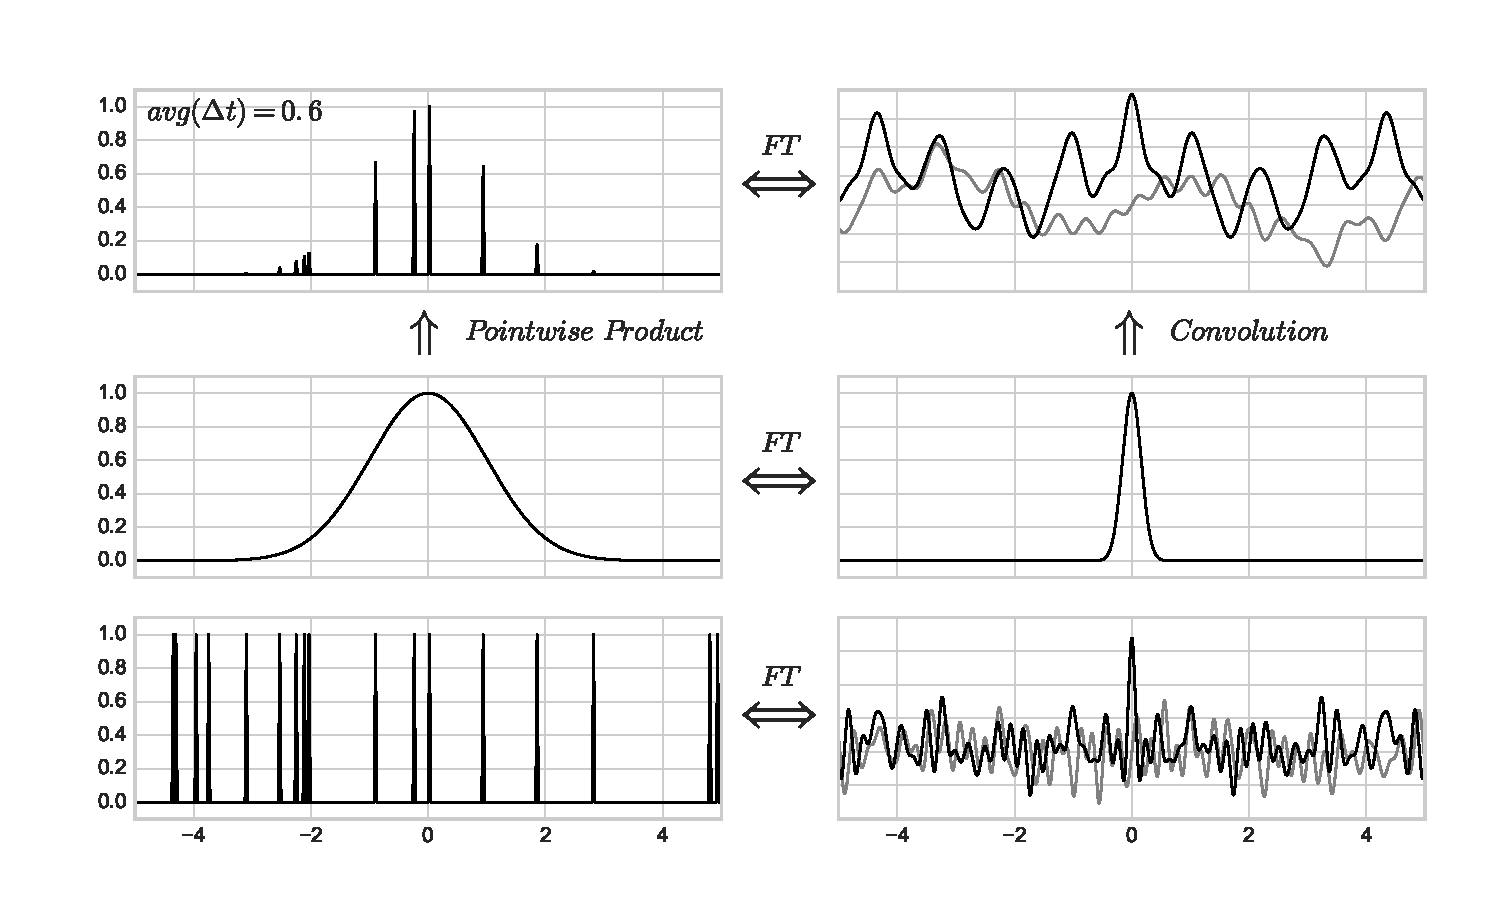
\includegraphics[width=\textwidth]{fig10_random_window}
  \caption{The effect of non-uniform sampling on the observed Fourier transform.
    These samples have the same average spacing as those in \fig{comb_window_1},
    but the lack of structure in observing window translates to a lack of
    structure in its transform, causing the observed transform to be ``noisy''.
    \figlabel{random_window}}
\end{figure}

One might hope that sampling the signal more densely might limit these problems,
and it does, but only to a degree.
\Fig{random_window_2} increases the density of observations by a factor of 10,
such that there are 200 total observations over the length-10 observing window.
The observed Fourier transform in this case is much more reflective of the
underlying signal, but still contains a degree of ``noise'' rooted in the
unstructured nature of the spacing between observations.


\begin{figure}[ht]
  \centering
  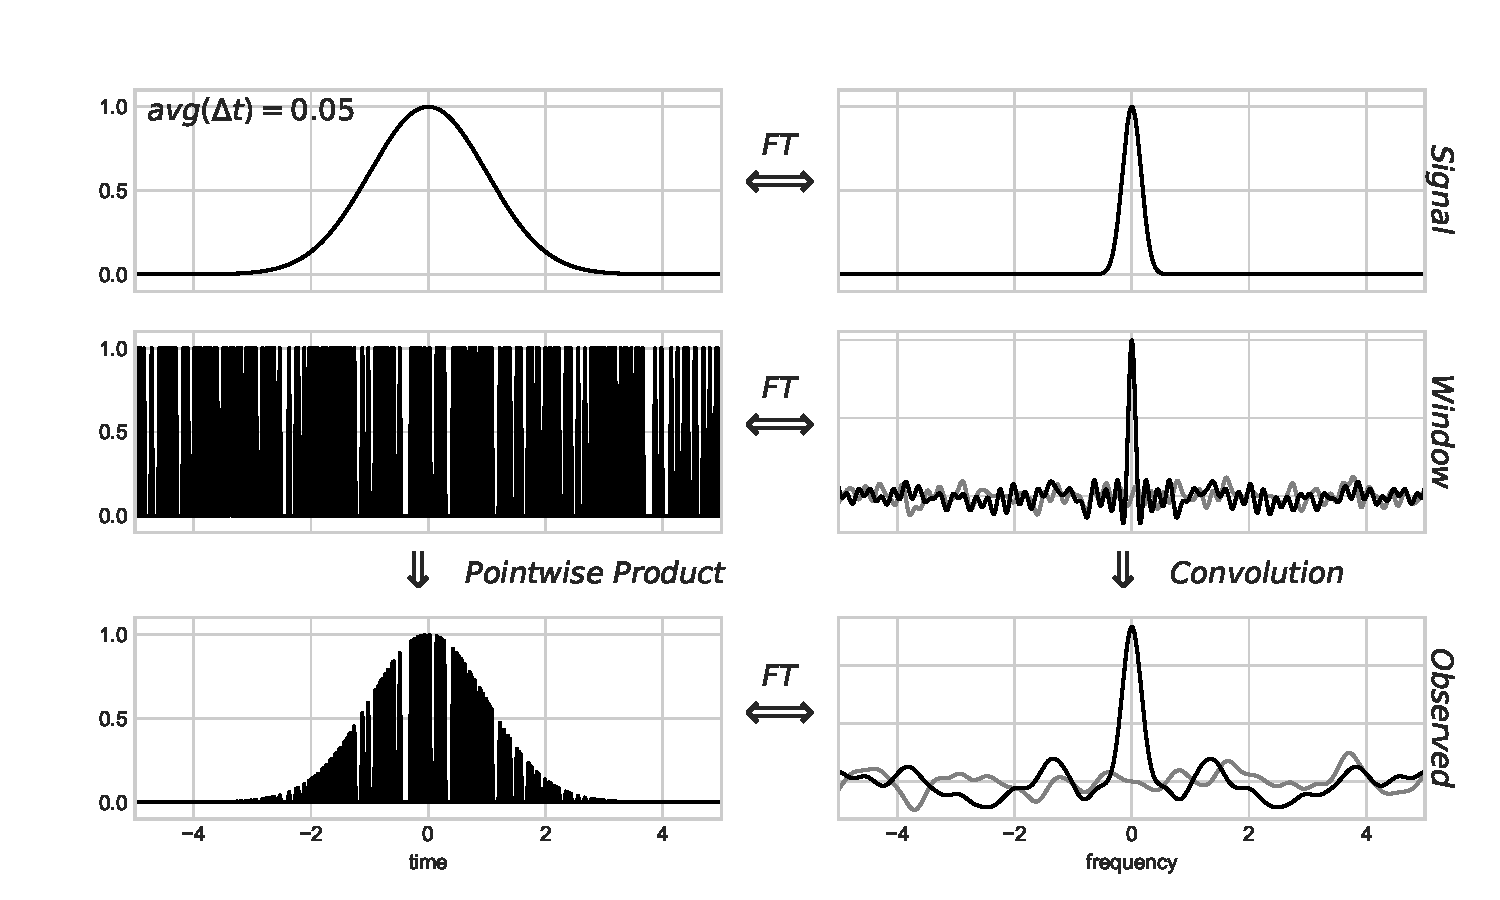
\includegraphics[width=\textwidth]{fig11_random_window_2}
  \caption{The effect of non-uniform sampling on the observed Fourier transform,
    with a factor of 10 more samples than \fig{random_window}.
    Even with very dense sampling of the function, the Fourier transform
    cannot be exactly recovered due to the 
    These samples have the same average spacing as those in \fig{comb_window_1},
    but the lack of structure in observing window translates to a lack of
    structure in its transform, causing the observed transform to be a
    ``noisy'' representation of the true transform
    \figlabel{random_window_2}}
\end{figure}

Since the observed transform is a well-defined convolution of the (unknown) true
transform and the (known) window transform, you might hope that we could
perform some sort of deconvolution operation to recover the result, but this
turns out not to be straightforward, as deconvolution (particularly in this
case where delta functions are involved) is an ill-posed problem without a
unique solution.

\subsection{Non-Uniform Periodogram}

From this non-uniform Fourier transform, it is straightforward to extend the
definition of the Schuster periodogram to the non-uniform case.
Plugging \eq{g-nonuniform} into the Fourier transform of \eq{FT-def}, in analogy to \eq{schuster-periodogram}, gives the following form of the power spectrum:
\begin{equation}
  P(f) = \frac{1}{N}\left|\sum_{n=1}^N g(t_n)e^{-2\pi i t_n} \right|^2
\end{equation}
Becuase it is derived from the Fourier transform of a non-uniformly sampled
function, this periodogram is subject to all the caveats mentioned here: in
particular, the periodogram measures the periodic content of the
{\it windowed signal} and thus reflects a convolution of the true signal
with a non-structured window function.
The resulting periodogram, then, can only be used as a qualitative approximation
of the true periodogram, and will only approach the true periodogram as the
number of observed samples gets very large.


\subsection{A Non-uniform Nyquist Limit?}

NO!!!

Examples: average \citep{NumRec, Horne86, Scargle82}, minimum \citep{Roberts87, Press89}, average of inverse time intervals \citep{Debosscher07},
time interval of measurement \citep{ICVG2014}, common multiple of observing time \citep{Eyer99}

\todo{Reference Figure 1 LINEAR data avg frequency vs computed period}


\citet{Scargle82} (citing the following: Beutler 1966, 1970; Masry \& Lui 1975; Higgins 1976; Wiley 1978; Gaster \& Roberts 1975, 1977; Kar, Hornkohl \& Farmer 1981; Ludeman 1981):
\begin{quote}
Error-free recovery of a band-limited signal [i.e.~reproduction of the entire function $X(t)$ from the samples $X(t_i)$] can be achieved with irregular sampling as long as the mean sampling rate exceeds the Nyquist rate (i.e. the average number of samples per unit time must exceed twice the highest frequency component in the signal).
\end{quote}


\citet{NumRec}: 
\begin{quote}
One guide to choosing $f_{hi}$ is to compare it with the Nyquist frequency $f_c$ which would obtain if the $N$ data points were evenly spaced over the same span $T$, that is $f_c = N/(2T)$. The accompanying program includes an input parameter {\tt hifac}, defined as $f_{hi}/f_{c}$.
\end{quote}

\citet{Press89}:
\begin{quote}
It is often meaningful to examine frequencies significantly higher than the
Nyquist frequency that would obtain if the same number of data points were
evenly spaced in the same total length of time. Some spectral information is
obtainable for frequencies all the way up to something like half the inverse
spacing of the {\it closest} spaced points.
\end{quote}

\citet{Roberts87}:
\begin{quote}
...for arbitrary $\{t_r\}$, the sampling theorem tells us nothing.
If the data samples are otherwise equally spaced but with missing
points, the theorem says that the data completely determine
a function whose FT is zero for $|v| > 1/(2\Delta_{max})$, where $\Delta_{max}$
is the {\it largest completely sampled} data spacing. However,
there are smaller spacings, and these certainly carry information
about frequencies greater than $1/(2\Delta_{max} )$; some information
is available about frequencies as high as
$1/(2\Delta_{min} )$, where $\Delta_{min}$ is the smallest spacing between data
points. Furthermore, if the $\{t_r\}$ are more or less randomly
distributed, so that a wide range ofspacings are present and
there is little redundancy in the spacing between various
points, tests have shown (Paper II) that significant information
is available on frequencies greater than $l/(2\Delta_{min})$.

Nonetheless, in the present paper we will restrict ourselves
to frequencies obeying
$\nu < \nu_{max} = 1/(2\Delta_{min})$.
\end{quote}

\citet{Horne86}:
\begin{quote}
The largest frequency we calculated was $\pi N-)/T$ which
is the traditional Nyquist frequency for evenly-spaced data. The Nyquist
frequency is not well defined for unevenly spaced signals, but it can serve as
a reasonable upper limit for the calculation.
\end{quote}

\citet{Debosscher07}:
\begin{quote}
For the highest frequency, we used the average of the inverse time intervals
between the measurements: $f_N = 0.5(1/\Delta T)$ as a pseudo
Nyquist frequency. Note that $f_N$ is equal to the Nyquist frequency
in the case of equidistant sampling. For particular cases,
an even higher upper limit can be used \citep[see][]{Eyer99}.
Our upper limit should be seen as a compromise between
the required resolution to allow a good fitting, and computation
time.
\end{quote}


\todo{Demonstrate recovery of a signal well beyond these limits (Is LINEAR sufficient?}


\subsection{Semi-structured Observing Windows}

\begin{itemize}
  \item Nightly (e.g. ground-based imaging)
  \item Uniform, but with missing data (e.g. Kepler)
\end{itemize}


\section{The Lomb-Scargle Periodogram}

\begin{itemize}
  \item ... is like a Schuster periodogram.
  \item ... is also like a least-squares sinusoid fit.
  \item ... reminder that it is a {\it windowed} power spectrum
\end{itemize}


\section{Using Lomb-Scargle Effectively}

\begin{itemize}
  \item Expected peak width
  \item How to choose the frequency grid
  \item Normalization and interpretation
\end{itemize}


\section{Uncertainties in Periods}

\begin{itemize}
  \item Peak Width and why it's a poor proxy
  \item False Alarm Probability and why it fails
  \item Baluev method and why it's not enough
  \item Motivation of Bootstrap

\end{itemize}



\section{Algorithmic Considerations}

\begin{itemize}
\item Press \& Rybicki method; show some benchmarks.
\item NFFT method
\end{itemize}



\section{Generalizations \& Challenges}

\begin{itemize}
\item Bayesian view is (almost always) not useful
\item Multiterm makes the true period fit better, but also bumps the background noise.
\end{itemize}


\section{Acknowledgements}

\citet{Astropy2013}

\bibliographystyle{apj}
\bibliography{PracticalLombScargle}

\end{document}
